\section{Mixing consistency levels in RedBlue consistency}
\label{sec:redblue}
%As mentioned before, to scale out the Internet services to meet their ever-growing user base, many
%recent storage systems have been proposed to replicate operations following a

In this section, we present a hybrid consistency model called RedBlue
consistency, where weakly consistent operations, labeled blue, can be executed at a
single replica and propagated in the background, with mostly no
coordination with concurrent actions at other replicas, while others, labeled red,
require a stronger consistency level and thus require cross-replica
coordination. RedBlue consistency is one of several systems that
propose labeling operations according to their consistency levels~\cite{Ladin1992LazyReplication, Singh2009Zeno,Li2012RedBlue,Pileus}, but improves on these systems by offering a precise method for labeling operations.

\begin{figure}[t!]
\centering
 \begin{minipage}[t]{0.45\columnwidth}
\centering
\subfloat[RedBlue order $O$ of operations]{
\centering
%\includegraphics[width=0.9\columnwidth]{figures/redblue/redblueOrder/redblueGlobalOrder.pdf}
\includegraphics[bb=0 0 206 140]{redblueGlobalOrder.pdf}
\label{fig:expositoryorder}
}
\end{minipage}
\hfill
 \begin{minipage}[t]{0.45\columnwidth}
\centering
\subfloat[Serializations of $O$]{
%\includegraphics[width=1.0\columnwidth]{figures/redblue/redblueOrder/redblueOrderSerial.pdf}
\includegraphics[bb=0 0 216 220]{redblueOrderSerial.pdf}
\label{fig:expositoryexecutionorder}
}
\end{minipage}
\caption{RedBlue order and serializations for a system spanning two
  sites. Operations marked with {\Large $\star$} are red, and
  operations marked with $\bigtriangleup$ are blue. Dotted arrows in \protect\subref{fig:expositoryorder} indicate the partial ordering of
operations. }
\label{fig:expositoryfigure}
\end{figure}

\subsection{Defining RedBlue consistency}

RedBlue consistency relies on three components: (1) a partitioning of operations into weakly consistent blue operations whose order of execution
can vary from site to site, and red operations that must
be executed in the same order at all sites, (2) a RedBlue order, which defines a partial order of
operations where red operations have to be ordered with respect to each other, and (3) a set of site-specific serializations (i.e., total orders)
in which the operations are locally applied. More precisely:

\begin{mydef}[RedBlue consistency]
A replicated system is {\em RedBlue consistent} if each site $i$ applies
operations according to a linear extension of a RedBlue order $O$ of the operations
that were invoked, where $O$ is a partial order among those operations with the requirement that red operations are totally ordered in $O$.
\label{def:rbct}
\end{mydef}

Figure~\ref{fig:expositoryfigure} shows a RedBlue order and two
serializations, i.e., the linear extensions of that order in which
operations are applied at two different sites. In systems where every operation is
labeled red, RedBlue consistency is equivalent to
serializability~\cite{Bernstein1987CCR}; in systems where every
operation is labeled blue, RedBlue consistency becomes a form of causal consistency~\cite{bayou,cops,
Mahajan2010Depot}, since the partial order conveys the necessary causality between operations.

When applying RedBlue consistency to an application, we would like to label all operations blue
to obtain best performance.
However, this could lead to state divergence and invariant violation, when operations are not commutative.
We describe a set of sufficient conditions to guide the classification of operations in order to safely use weak consistency
when possible.

%When applying RedBlue consistency
%to an application, the challenge is that we cannot arbitrarily label operations as blue (weakly consistent), since that might lead to
%breaking state convergence and invariant preservation. Therefore, to safely use blue operations, we must come up with a %set of sufficient conditions to guide the classification, which will
%be described next.

\subsection{Ensuring state convergence}
In the context of RedBlue consistency, we can formalize state convergence as follows:

\begin{mydef}[State convergence]
A RedBlue consistent system is state convergent if all serializations of
the underlying RedBlue order $O$ reach the same state $S$ w.r.t.\ any initial state $S_0$.
\end{mydef}

To find a correct labeling for maintaining state convergence while providing low latency access, we describe a
simple banking example, in which users may share an account that is modified
via three operations, namely {\tt deposit}, {\tt withdraw} and {\tt accrueinterest}\footnote{{\tt accrueinterest}
computes a new balance by multiplying the old balance value and (1 + {\tt interest rate}).}. Keeping in mind that one of the goals of RedBlue consistency is to make the target service as fast as possible, we tentatively
label all these operations blue. According to this labeling result, we construct a RedBlue order of deposits and interest accruals made by two users Alice and Bob and two possible serializations applied at both branches
of the bank, as shown in Figure~\ref{fig:bankexample}. This example shows that the labeling of these operations as described is not state convergent. This is because
RedBlue consistency allows the two sites to execute blue operations in a different order, but
two of the blue operations in the example are non-commutative, namely
{\tt deposit} and {\tt accrueinterest}. To prevent this situation, a sufficient condition to guarantee
state convergence in a system supporting RedBlue consistency is that every blue operation commutes with all other operations, blue or red.

\begin{figure}[t]
\centering
\begin{minipage}[t]{0.46\columnwidth}
\centering
\subfloat[\sf RedBlue order $O$ of operations issued by Alice and Bob ]{
%\includegraphics[width=0.9\columnwidth]{figures/redblue/redblueOrder/redblueOrderBank.pdf}
\includegraphics[bb=0 0 222 30]{redblueOrderBank.pdf}
\label{fig:simplebankrbo}
}
\end{minipage}
\hfill
\begin{minipage}[t]{0.46\columnwidth}
\centering
\subfloat[\sf Serializations of $O$ leading to diverged state]{
%\includegraphics[width=1.0\columnwidth]{figures/redblue/redblueOrder/redblueOrderBankSerial.pdf}
\includegraphics[bb=0 0 222 90]{redblueOrderBankSerial.pdf}
\label{fig:divergestate}
}
\end{minipage}
\caption{A RedBlue consistent account with initial balance of 100 and final diverged state}.
%\changebars{}{ (a) \RBo\ of
%  \operations\ issued by Alice and Bob. (b) Divergent causal serializations.}}
\label{fig:bankexample}
\end{figure}

However, when applying this condition to the banking example, it implies that we need to label all three operations red
({\tt deposit}, {\tt withdraw} and {\tt accrueinterest}).
This is equivalent to running the system under serializability, which requires coordination across replicas for executing all these operations.
To address the problem that it is difficult to find operations that commute with all other operations in the system, we observe that, in many cases,
while operations may not be commutative, we
can make the changes they induce on the system state to commute. In
the banking example, we can engineer {\tt accrueinterest} commute with the remaining two operations
by first computing the amount of interested accrued at the primary replica and then treating that value as a deposit.


To exploit this observation and increase operation commutativity, we propose a change to our
original system model,
where we split each original application operation $u$
into two components: a {\em generator operation} $g_u$ with no
side-effects, which is executed only at the primary site against some
system state $S$ and produces a {\em shadow operation} $h_u(S)$,
which is executed at every site (including the primary site). The
generator operation decides which state transitions should be made
while the shadow operation applies the transitions in a
state-indep\-endent manner.

\subsection{Preserving invariants}
%While the concept of shadow operation helps produce more commutative operations, it
%Concurrency introduces the problem of breaking application invariants. 
Although the concept of shadow operation helps produce more commutative operations, labeling too many
shadow operations as blue may introduce the problem of breaking application invariants. In the banking example, assuming that the shared bank account has an initial balance of $100$, if both Alice and Bob withdraw $70$ and $60$ respectively,
the final balance would be $-30$. This violates the
invariant that a bank balance should never be negative. To determine which shadow 
operations can be safely labeled blue, we begin by defining that a
shadow operation is invariant safe if, when applied to a valid state, it always transitions
the system into another valid state. This allows us to define the following
sufficient condition: a RedBlue consistent system preserves invariants (meaning that all its sites are always in valid states) if all shadow operations that are not invariant safe are labeled red (i.e., strongly consistent).

\if 0
\begin{theorem}[Invariant preservation]
A RedBlue consistent system preserves invariants (meaning that all its sites are always in valid states) if all operations that are not invariant safe are labeled red (i.e., strongly consistent).
\end{theorem}
\fi

\subsection{What can be blue?  What must be red?}
\label{ch:redblue:sect:labelmethod}
In summary, the two conditions above lead to the following procedure for deciding
which shadow operations can be
blue or must be red if a RedBlue consistent system is to provide both
state convergence and invariant preservation:
\begin{enumerate}%[leftmargin=0cm,itemindent=.5cm,labelwidth=\itemindent,labelsep=0cm,align=left]
\item For any pair of non-commutative shadow operations $h_u$ and $h_v$, label both $h_u$ and $h_v$ red.
\item For any shadow operation $h_u$ that is not invariant safe,
label $h_u$ red.
\item Label all remaining shadow operations blue.
\end{enumerate}

